\chapter{Metodologia}
\label{cap:03}

% Este capítulo visa descrever a metodologia empregada no desenvolvimento do GUY - apresentando desde o Panorama Geral da Pesquisa até o desenvolvimento da aplicação em si.

Este capítulo apresenta o método da pesquisa e o processo de desenvolvimento da extensão GUY. Primeiro, delimita-se o objeto de análise e a forma de avaliação; em seguida, descrevem-se as atividades de construção da ferramenta, sem confundir o procedimento de pesquisa com as decisões de implementação.

\section{Método da Pesquisa}
\label{sec:metodo_pesquisa}

Trata-se de uma pesquisa aplicada, de caráter exploratório e descritivo, conduzida por meio da construção e da avaliação técnica de uma ferramenta de análise estática. O objeto de análise é o código Python apresentado ao GUY no VS Code, nos escopos de arquivo, seleção ou função atual. A avaliação não envolve a execução dos programas: verifica a correspondência entre as estruturas de controle reconhecidas, o GFC construído e o valor da Complexidade Ciclomática.

Para a validação, foram utilizados os três arquivos de exemplo disponíveis em \texttt{src/examples/}, que representam diferentes combinações de estruturas de controle em Python. Para cada exemplo, os nós, as arestas, as decisões, os componentes e os caminhos independentes foram confrontados com uma reconstrução manual baseada na convenção de modelagem do GFC e com a fórmula de $V(G)$. Portanto, os resultados sustentam conclusões apenas para esses exemplos e para o escopo implementado.

\section{Panorama Geral da Pesquisa}
% Elaborar uma ilustração visual, no esquema da Perspectiva do Produto do Documento de Visão e apresentar e explicar a figura aqui.
% Esta figura tem que trazer o contexto principal da sua pesquisa, onde está inserido, envolvidos, benefícios, fluxo, etc...
Como ilustrado na Figura \ref{fig:fluxo_GUY}, o GUY permite que programadores gerem Grafos de Fluxo de Controle (GFCs) a partir do arquivo aberto no \textit{Visual Studio Code} (VS Code). Com isso, a extensão apoia a compreensão da lógica interna do código e o planejamento de testes estruturais durante o desenvolvimento.

\begin{figure}[htbp]
\centering
\caption{Fluxo de funcionamento da ferramenta proposta.}
% Placeholder para o desenho do grafo
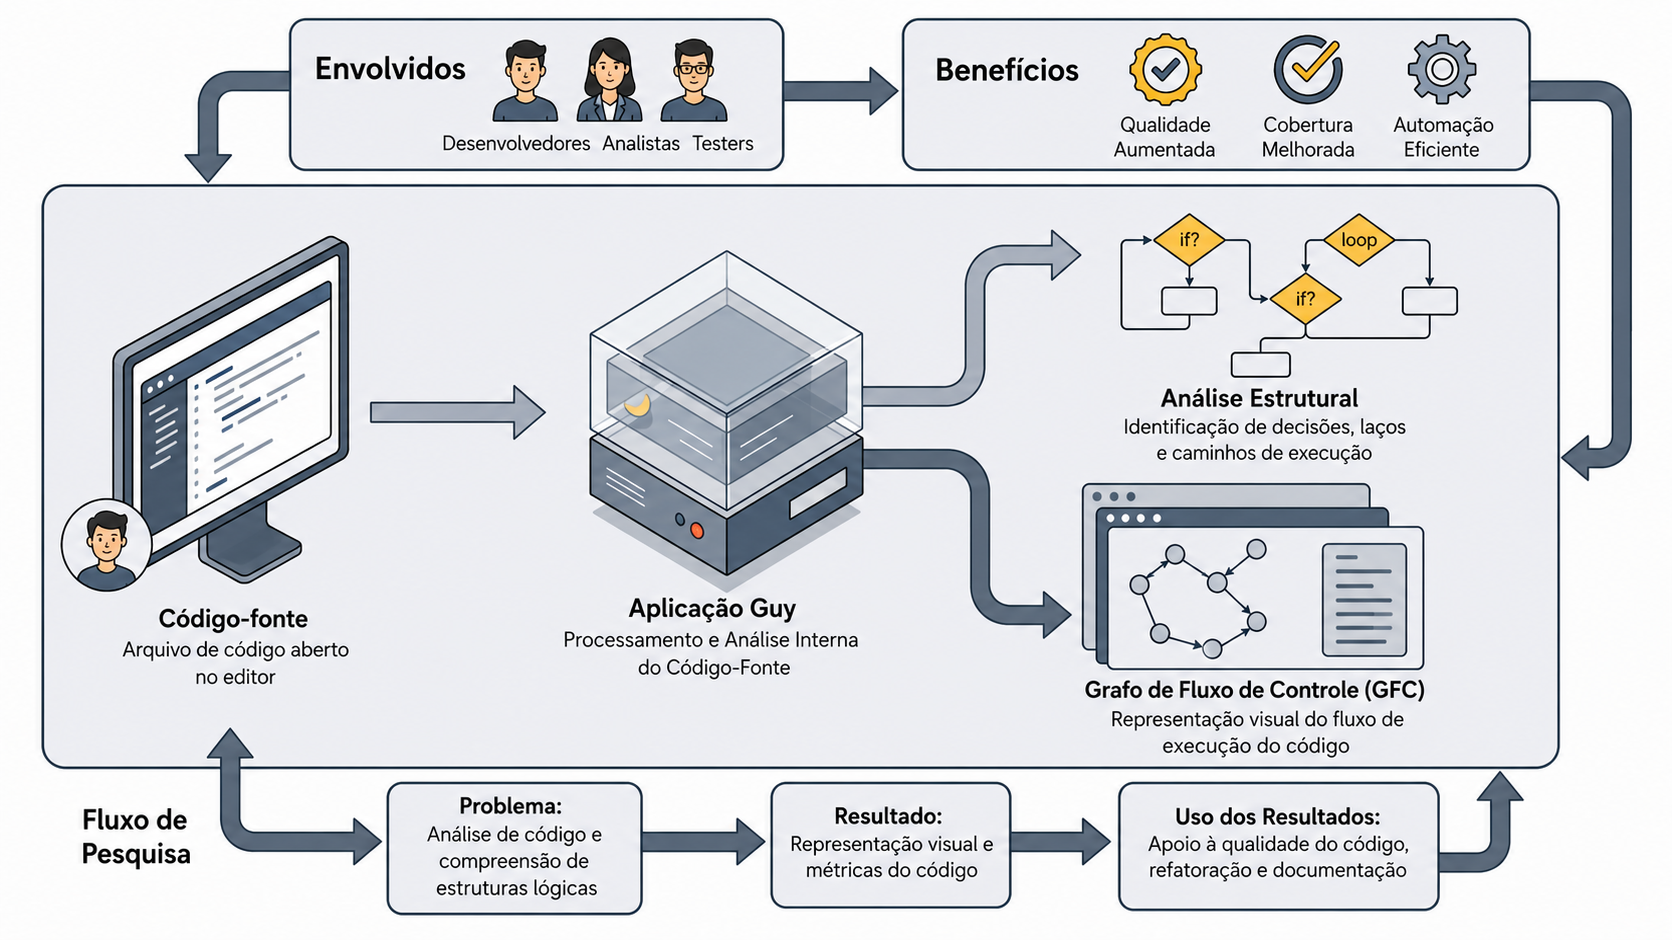
\includegraphics[width=0.75\linewidth]{imagens/fluxos/fluxo_guy.png}

\fonte{Elaborada pelo autor (2025).}
\label{fig:fluxo_GUY}

\end{figure}

A ferramenta é acionada a partir do arquivo de código-fonte aberto no editor. Em seguida, o núcleo de processamento do GUY executa a análise estática local, mapeia as estruturas lógicas do algoritmo e constrói a representação visual do Grafo de Fluxo de Controle. Essa representação permite identificar os nós de decisão e os caminhos de execução possíveis no trecho analisado.

Com o GFC estruturado, o desenvolvedor passa a visualizar os caminhos independentes do algoritmo. Essa visualização integrada auxilia desenvolvedores e analistas de qualidade (\textit{testers}) na identificação dos fluxos que podem orientar a elaboração de casos de teste estruturais.



\section{Etapas para o Desenvolvimento da Ferramenta Proposta}
% Elaborar uma figura de passo a passo para definir as etapas para o desenvolvimento e depois explicar detalhadamente como cada uma das etapas serão desenvolvidas.
O desenvolvimento do GUY seguiu uma abordagem de pesquisa aplicada, de caráter exploratório e descritivo, associada à construção experimental de uma ferramenta de apoio à análise estrutural de código. As principais fases do projeto estão sumarizadas na Figura \ref{fig:fluxo_met_GUY}.

\begin{figure}[H]
\centering
\caption{Fluxo das etapas metodológicas para o desenvolvimento.}
% Placeholder para o desenho do grafo
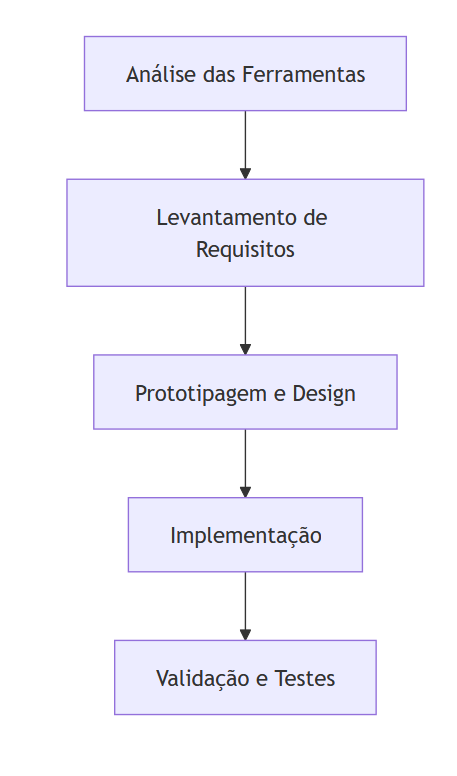
\includegraphics[width=0.35\linewidth]{imagens/fluxos/fluxo_met_guy.png}

\fonte{Elaborada pelo autor.}
\label{fig:fluxo_met_GUY}

\end{figure}

A metodologia relaciona fundamentação teórica, levantamento de requisitos, concepção da solução, implementação e validação. O fluxo apresentado na Figura \ref{fig:fluxo_met_GUY} inicia-se pela investigação de ferramentas correlatas, passa pela definição dos requisitos e da arquitetura da solução e termina com a codificação e a avaliação das funcionalidades.

A análise das ferramentas correlatas apresentadas no trabalho -- SonarQube, Codacy e ESLint -- foi qualitativa e considerou os recursos observados de análise ou qualidade de código e a forma de apresentação dos diagnósticos. Essa seleção não pretende representar todo o mercado nem permite conclusões sobre superioridade. Em seguida, a prototipagem orientou a implementação, e os resultados foram avaliados por meio da comparação entre os grafos e valores de complexidade gerados pela ferramenta e os resultados esperados para os exemplos analisados. Cada bloco apresentado na Figura \ref{fig:fluxo_met_GUY} representa uma etapa do desenvolvimento, detalhada a seguir:

\begin{enumerate}
\item \textbf{Análise de Ferramentas Correlatas:} foram observadas as funcionalidades documentadas para SonarQube, Codacy e ESLint, com foco na relação dessas ferramentas com análise ou qualidade de código e na apresentação de seus diagnósticos.
\item \textbf{Levantamento de Requisitos:} foram definidos os requisitos funcionais e não funcionais necessários para a extensão, incluindo execução local, geração do grafo, cálculo de métricas e integração com o editor.
\item \textbf{Prototipagem e \textit{Design}:} foram elaborados os \textit{wireframes} e a organização da interface, considerando a visualização do grafo em uma janela lateral do VS Code.
\item \textbf{Implementação (Codificação):} a extensão foi desenvolvida em TypeScript para o VS Code. O analisador sintático de Python utiliza Tree-sitter por meio de WebAssembly; a interface interativa é renderizada em uma \textit{Webview} com React, \texttt{@xyflow/react} e \texttt{@dagrejs/dagre}.
\item \textbf{Validação e Testes:} foram realizadas verificações funcionais e comparações entre os resultados gerados pela ferramenta e os grafos e valores de complexidade esperados para os códigos analisados.
\end{enumerate}

Os resultados obtidos são apresentados no Capítulo 4, com o detalhamento da implementação do GUY e da validação das funcionalidades desenvolvidas.
